% \documentclass{standalone}
\documentclass[multi=my,crop]{standalone}
\usepackage{graphicx}
\usepackage{amsmath}
\usepackage{amssymb}
\usepackage{booktabs}
\usepackage{lipsum}
\usepackage{tikz}
\usepackage{relsize}
\usepackage{pgfplots}
\usepackage{pgfplotstable}
\usepackage{subcaption}
\usepackage{multicol}

\begin{document}
    \begin{my}
        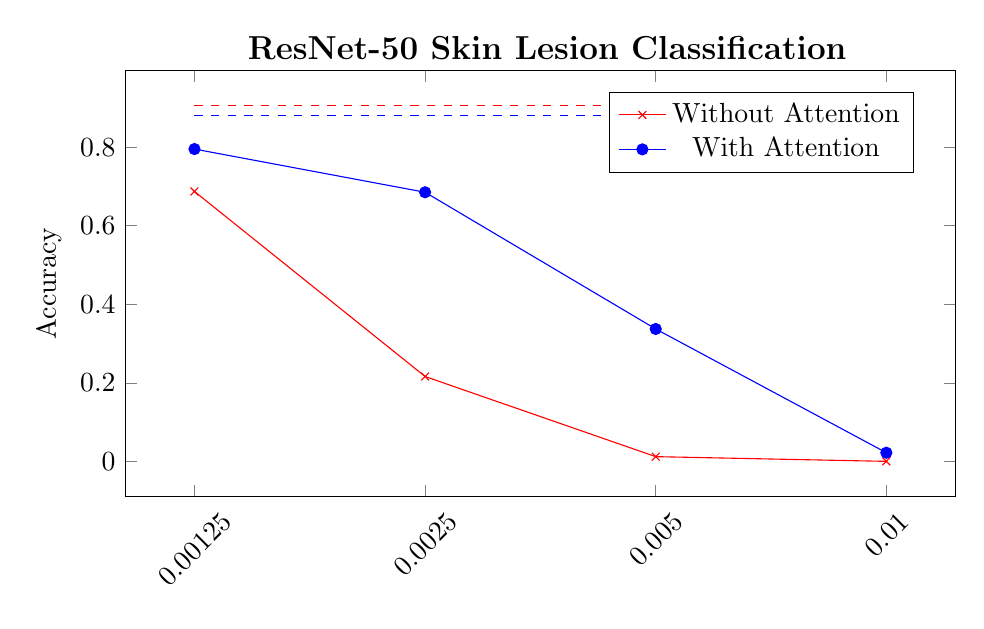
\begin{tikzpicture}
            \begin{axis}[xtick={0, 0.00125, 0.0025, 0.005, 0.01, 0.02, 0.04, 0.08, 0.16, 0.32}, x tick label style={rotate=45, log ticks with fixed point},xmode=log, log basis x=2, xlabel=, ylabel=Accuracy, width=\linewidth, height=7cm,legend style={at={(0.95,0.95)},anchor=north east}]
                
                \addplot[color=red,mark=x] coordinates {
                    (0.00125, 0.687)
                    (0.0025, 0.216)
                    (0.005, 0.012)
                    (0.01, 0)
                };
                
                \addplot[color=blue,mark=*] coordinates {
                    (0.00125, 0.795)
                    (0.0025, 0.685)
                    (0.005, 0.337)
                    (0.01, 0.022)
                };
            
                \addplot[color=red, domain=0.00125:0.01, dashed]{0.905};
                \addplot[color=blue, domain=0.00125:0.01, dashed]{0.880};
                
                \legend{Without Attention,With Attention}
            \end{axis}
            \node[above,font=\large\bfseries] at (current bounding box.north) {$\,\,\,\,\,\,\,\,\,\,\,\,\,\,\,\,\,\,\,\,$ResNet-50 Skin Lesion Classification};
        \end{tikzpicture}
    \end{my}
    \begin{my}
        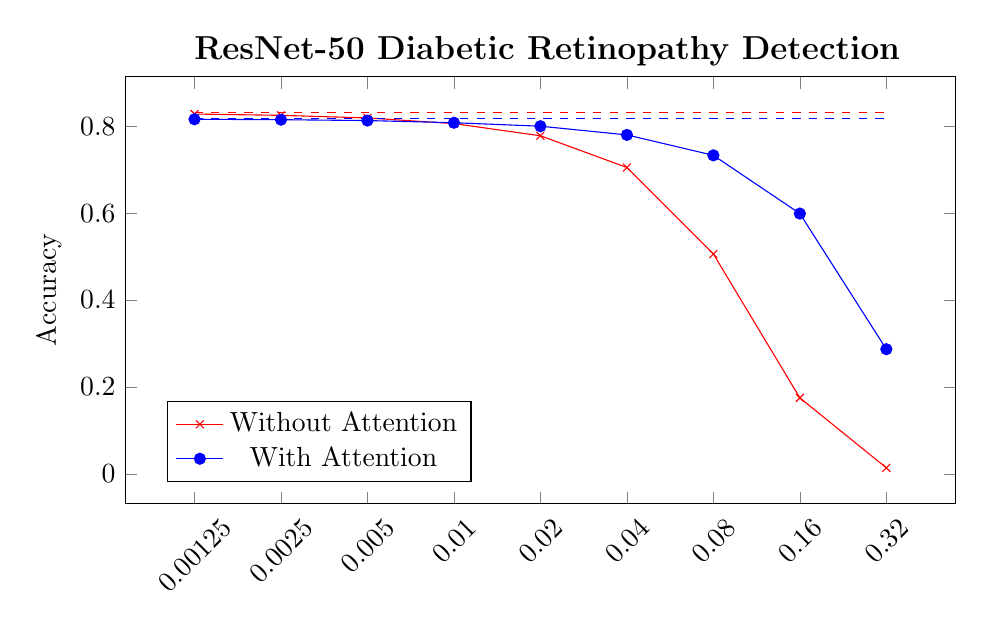
\begin{tikzpicture}
            \begin{axis}[xtick={0, 0.00125, 0.0025, 0.005, 0.01, 0.02, 0.04, 0.08, 0.16, 0.32}, x tick label style={rotate=45, log ticks with fixed point},xmode=log, log basis x=2, xlabel=, ylabel=Accuracy, width=\linewidth, height=7cm,legend style={at={(0.05,0.05)},anchor=south west}]
                
            \addplot[color=red,mark=x] coordinates {
              (0, 0.832)
              (0.00125, 0.828)
              (0.0025, 0.825)
              (0.005, 0.819)
              (0.01, 0.806)
              (0.02, 0.778)
              (0.04, 0.705)
              (0.08, 0.506)
              (0.16, 0.175)
              (0.32, 0.014)
            };
            
            \addplot[color=blue,mark=*] coordinates {
              (0, 0.818)
              (0.00125, 0.816)
              (0.0025, 0.815)
              (0.005, 0.813)
              (0.01, 0.808)
              (0.02, 0.8)
              (0.04, 0.780)
              (0.08, 0.733)
              (0.16, 0.599)
              (0.32, 0.287)
            };
      
            \addplot[color=red, domain=0.00125:0.32, dashed]{0.832};
            \addplot[color=blue, domain=0.00125:0.32, dashed]{0.818};
            
            \legend{Without Attention,With Attention}
            \end{axis}
            \node[above,font=\large\bfseries] at (current bounding box.north) {$\,\,\,\,\,\,\,\,\,\,\,\,\,\,\,\,\,\,\,\,$ResNet-50 Diabetic Retinopathy Detection};
            \end{tikzpicture}
    \end{my}
    \begin{my}
        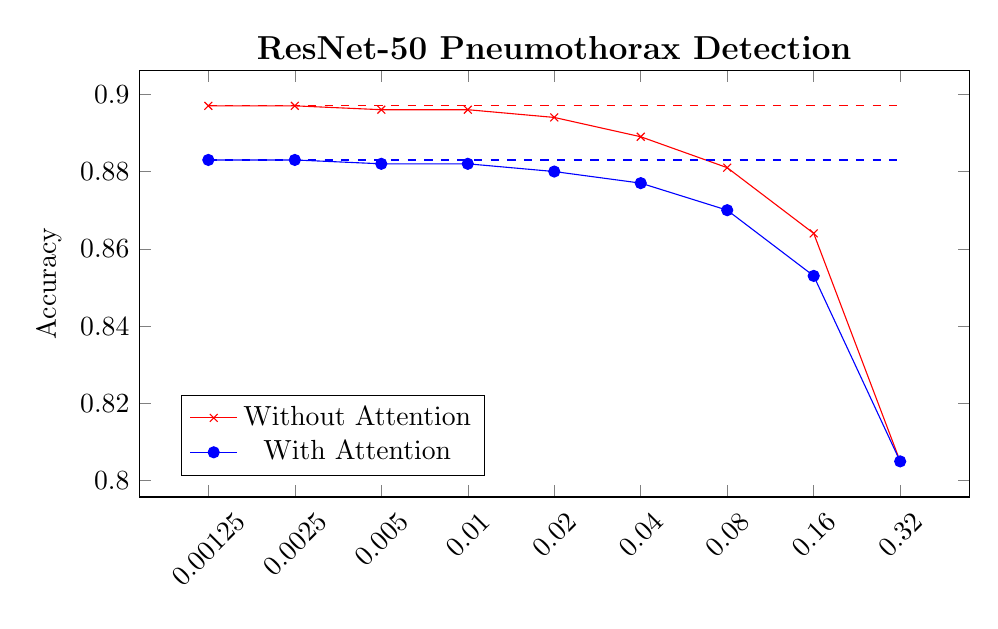
\begin{tikzpicture}
            \begin{axis}[xtick={0, 0.00125, 0.0025, 0.005, 0.01, 0.02, 0.04, 0.08, 0.16, 0.32}, x tick label style={rotate=45, log ticks with fixed point},xmode=log, log basis x=2, xlabel=, ylabel=Accuracy, width=\linewidth, height=7cm,legend style={at={(0.05,0.05)},anchor=south west}]
                
            \addplot[color=red,mark=x] coordinates {
              (0.00125, 0.897)
              (0.0025, 0.897)
              (0.005, 0.896)
              (0.01, 0.896)
              (0.02, 0.894)
              (0.04, 0.889)
              (0.08, 0.881)
              (0.16, 0.864)
              (0.32, 0.805)
            };
            
            \addplot[color=blue,mark=*] coordinates {
              (0.00125, 0.883)
              (0.0025, 0.883)
              (0.005, 0.882)
              (0.01, 0.882)
              (0.02, 0.880)
              (0.04, 0.877)
              (0.08, 0.870)
              (0.16, 0.853)
              (0.32, 0.805)
            };
      
            \addplot[color=red, domain=0.00125:0.32, dashed]{0.897};
            \addplot[color=blue, domain=0.00125:0.32, dashed]{0.883};
            
            \legend{Without Attention,With Attention}
            \end{axis}
            \node[above,font=\large\bfseries] at (current bounding box.north) {$\,\,\,\,\,\,\,\,\,\,\,\,\,\,\,\,\,\,\,\,$ResNet-50 Pneumothorax Detection};
            \end{tikzpicture}
    \end{my}
    \begin{my}
        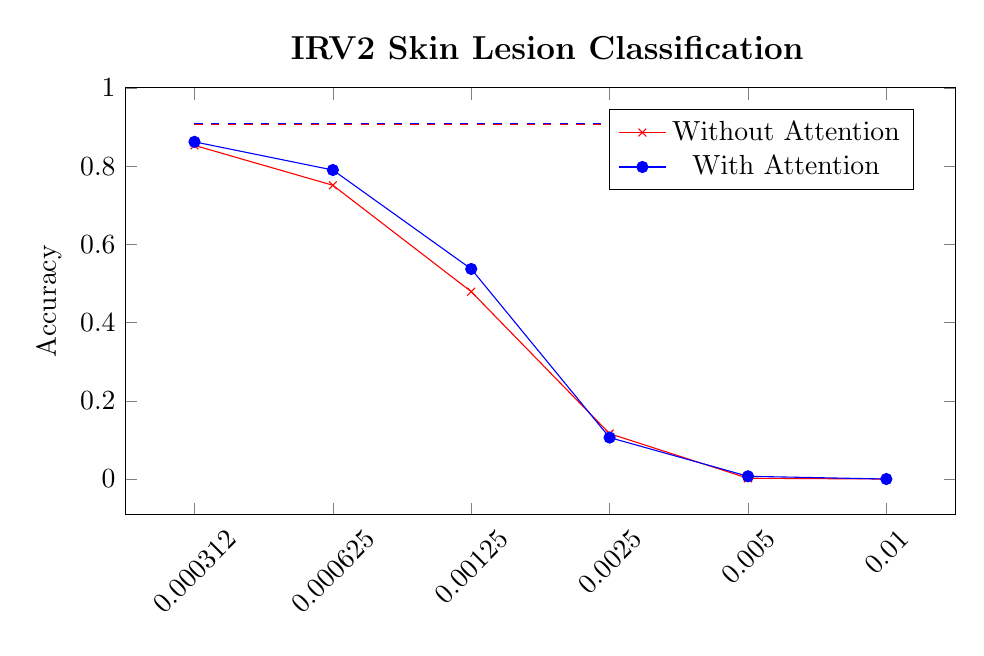
\begin{tikzpicture}
            \begin{axis}[xtick={0, 0.0003125, 0.000625, 0.00125, 0.0025, 0.005, 0.01}, x tick label style={rotate=45, log ticks with fixed point},xmode=log, log basis x=2, xlabel=, ylabel=Accuracy, width=\linewidth, height=7cm,legend style={at={(0.95,0.95)},anchor=north east}]
                
            \addplot[color=red,mark=x] coordinates {
              (0.0003125, 0.853)
              (0.000625, 0.751)
              (0.00125, 0.479)
              (0.0025, 0.116)
              (0.005, 0.002)
              (0.01, 0.0)
            };
            
            \addplot[color=blue,mark=*] coordinates {
              (0.0003125, 0.862)
              (0.000625, 0.790)
              (0.00125, 0.537)
              (0.0025, 0.106)
              (0.005, 0.007)
              (0.01, 0.0)
            };
      
            \addplot[color=red, domain=0.0003125:0.01, dashed]{0.906};
            \addplot[color=blue, domain=0.0003125:0.01, dashed]{0.909};
            
            \legend{Without Attention,With Attention}
            \end{axis}
            \node[above,font=\large\bfseries] at (current bounding box.north) {$\,\,\,\,\,\,\,\,\,\,\,\,\,\,\,\,\,\,\,\,$IRV2 Skin Lesion Classification};
            \end{tikzpicture}
    \end{my}
    \begin{my}
        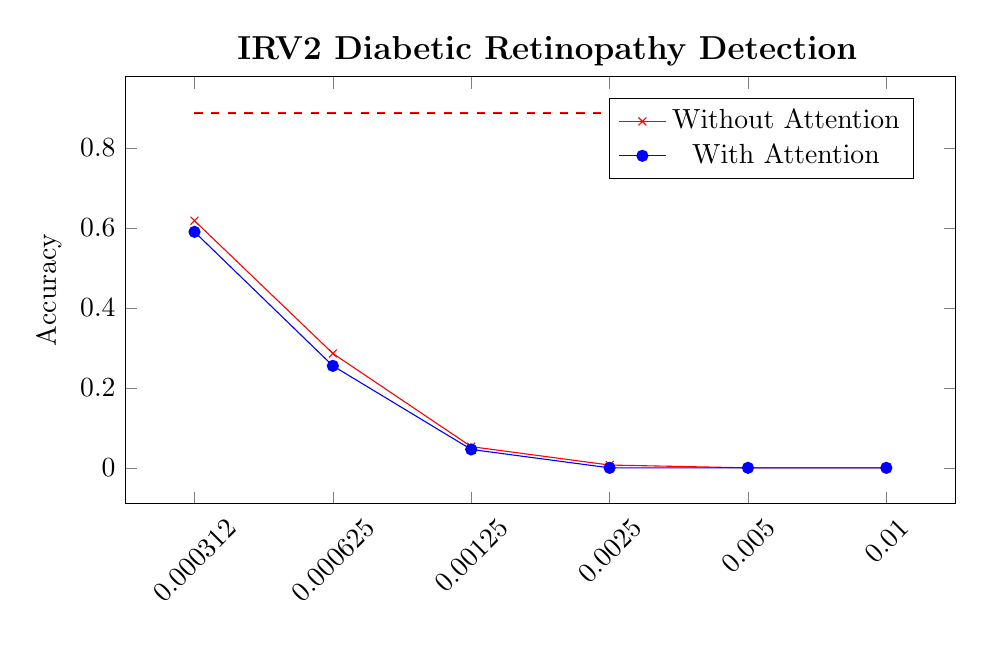
\begin{tikzpicture}
            \begin{axis}[xtick={0, 0.0003125, 0.000625, 0.00125, 0.0025, 0.005, 0.01}, x tick label style={rotate=45, log ticks with fixed point},xmode=log, log basis x=2, xlabel=, ylabel=Accuracy, width=\linewidth, height=7cm,legend style={at={(0.95,0.95)},anchor=north east}]
            
            \addplot[color=red,mark=x] coordinates {
              (0.0003125, 0.618)
              (0.000625, 0.286)
              (0.00125, 0.053)
              (0.0025, 0.007)
              (0.005, 0.0)
              (0.01, 0.0)
            };
            
            \addplot[color=blue,mark=*] coordinates {
              (0.0003125, 0.590)
              (0.000625, 0.255)
              (0.00125, 0.046)
              (0.0025, 0.0)
              (0.005, 0.0)
              (0.01, 0.0)
            };
      
            \addplot[color=red, domain=0.0003125:0.01, dashed]{0.889};
            \addplot[color=blue, domain=0.0003125:0.01, dashed]{0.887};
            
            \legend{Without Attention,With Attention}
            \end{axis}
            \node[above,font=\large\bfseries] at (current bounding box.north) {$\,\,\,\,\,\,\,\,\,\,\,\,\,\,\,\,\,\,\,\,$IRV2 Diabetic Retinopathy Detection};
            \end{tikzpicture}
    \end{my}
    \begin{my}
        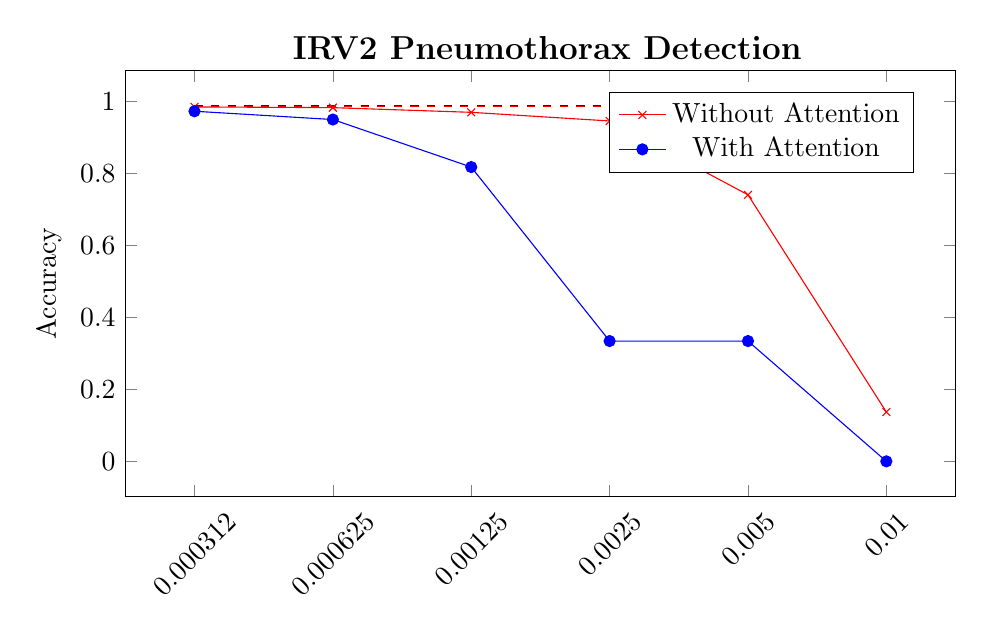
\begin{tikzpicture}
            \begin{axis}[xtick={0, 0.0003125, 0.000625, 0.00125, 0.0025, 0.005, 0.01}, x tick label style={rotate=45, log ticks with fixed point},xmode=log, log basis x=2, xlabel=, ylabel=Accuracy, width=\linewidth, height=7cm,legend style={at={(0.95,0.95)},anchor=north east}]
      
            \addplot[color=red,mark=x] coordinates {
              (0.0003125, 0.984)
              (0.000625, 0.982)
              (0.00125, 0.969)
              (0.0025, 0.945)
              (0.005, 0.740)
              (0.01, 0.137)
            };
            
            \addplot[color=blue,mark=*] coordinates {
              (0.0003125, 0.972)
              (0.000625, 0.949)
              (0.00125, 0.817)
              (0.0025, 0.334)
              (0.005, 0.334)
              (0.01, 0.0)
            };
      
            \addplot[color=red, domain=0.0003125:0.01, dashed]{0.986};
            \addplot[color=blue, domain=0.0003125:0.01, dashed]{0.987};
            
            \legend{Without Attention,With Attention}
            \end{axis}
            \node[above,font=\large\bfseries] at (current bounding box.north) {$\,\,\,\,\,\,\,\,\,\,\,\,\,\,\,\,\,\,\,\,$IRV2 Pneumothorax Detection};
            \end{tikzpicture}
    \end{my}
\end{document}